\documentclass[tikz,border=5pt,10pt]{standalone}
\usepackage{tikz}
\usetikzlibrary{calc}
\usepackage{pgf,xcolor}
\usepackage{eulervm}
\usepackage{booktabs,rotating,multirow,caption}
\usepackage{makecell}
\usetikzlibrary{automata}
\usetikzlibrary{arrows}
\usepackage{mathdots}
\usetikzlibrary{decorations.pathreplacing}
\usetikzlibrary{backgrounds}
\newcommand*\packet[1]{\tikz[baseline=(char.base)]{
            \node[thick,fill=white,shape=rectangle,draw,inner sep=2.5pt] (char) {#1};}}
\begin{document}
\begin{small}{\sffamily
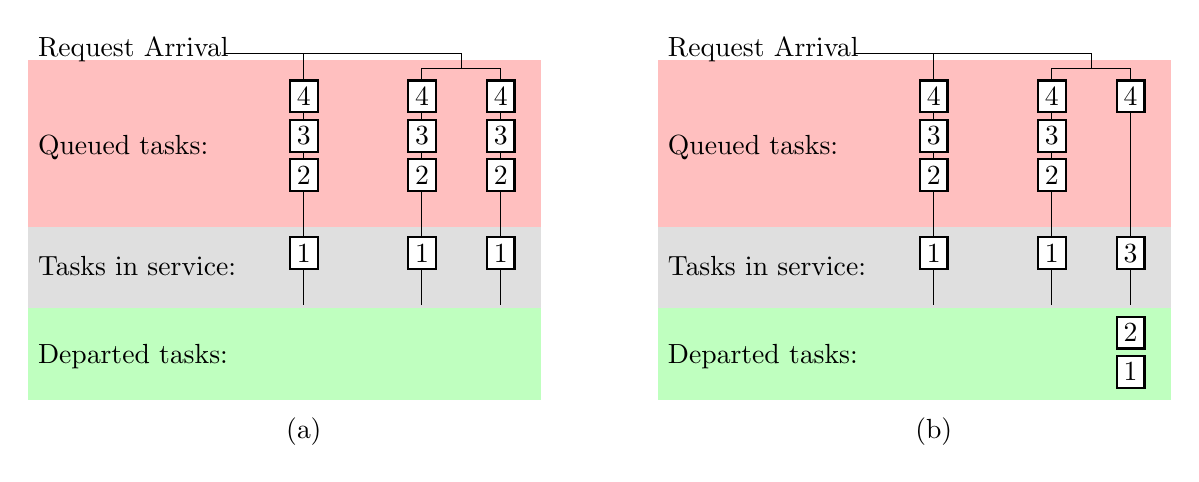
\begin{tikzpicture} %[line width=1.1pt]
\draw [fill=gray!25,gray!25] (-1.5,-2.01) rectangle (5,-3.05); 
\draw [fill=red!25,red!25] (-1.5,0.1) rectangle (5,-2); 
\draw [fill=green!25,green!25] (-1.5,-3.05) rectangle (5,-4.2); 
\node [right] at (-1.5,0.25) {Request Arrival};
\draw (1,0.2) -- (4,0.2);
% sys
\draw (2,0.2) -- (2,-3);
% waiting
\node at (2,-1.35) {$\packet{2}$};
\node at (2,-0.85) {$\packet{3}$};
\node at (2,-0.35) {$\packet{4}$};
% in service
\node [below] at (2,-2) {$\packet{1}$};
% repair
\draw (4,0.2) --(4,0);
\draw (3.5,-3)--(3.5,0)--(4.5,0)--(4.5,-3);
% repair waiting
\node at (3.5,-1.35) {$\packet{2}$};
\node at (3.5,-0.85) {$\packet{3}$};
\node at (3.5,-0.35) {$\packet{4}$};
\node at (4.5,-1.35) {$\packet{2}$};
\node at (4.5,-0.85) {$\packet{3}$};
\node at (4.5,-0.35) {$\packet{4}$};
% repair in service
\node [below] at (3.5,-2) {$\packet{1}$};
\node [below] at (4.5,-2) {$\packet{1}$};
%
\node [right] at (-1.5,-1) {Queued tasks:};
\node [right] at (-1.5,-3.65) {Departed tasks:};
\node [right] at (-1.5,-2.5) {Tasks in service:};
\node at (2.,-4.6) {\normalsize (a)};
%
\begin{scope}[xshift=8cm]
\draw [fill=gray!25,gray!25] (-1.5,-2.01) rectangle (5,-3.05); 
\draw [fill=red!25,red!25] (-1.5,0.1) rectangle (5,-2); 
\draw [fill=green!25,green!25] (-1.5,-3.05) rectangle (5,-4.2); 
\node [right] at (-1.5,0.25) {Request Arrival};
\draw (1,0.2) -- (4,0.2);
% sys
\draw (2,0.2) -- (2,-3);
% waiting
\node at (2,-0.35) {$\packet{4}$};
\node at (2,-0.85) {$\packet{3}$};
\node at (2,-1.35) {$\packet{2}$};
% in service
\node [below] at (2,-2) {$\packet{1}$};
% repair
\draw (4,0.2) --(4,0);
\draw (3.5,-3)--(3.5,0)--(4.5,0)--(4.5,-3);
% waiting
\node at (3.5,-0.35) {$\packet{4}$};
\node at (3.5,-0.85) {$\packet{3}$};
\node at (3.5,-1.35) {$\packet{2}$};
\node at (4.5,-0.35) {$\packet{4}$};
% in service
\node [below] at (3.5,-2) {$\packet{1}$};
\node [below] at (4.5,-2) {$\packet{3}$};
% departed
\node at (4.5,-3.35) {$\packet{2}$};
\node at (4.5,-3.85) {$\packet{1}$};
%
\node [right] at (-1.5,-1) {Queued tasks:};
\node [right] at (-1.5,-3.65) {Departed tasks:};
\node [right] at (-1.5,-2.5) {Tasks in service:};
\node at (2.,-4.6) {\normalsize (b)};
\end{scope}
\end{tikzpicture}
}\end{small}
\end{document}